\documentclass[pdftex,twoside,a4paper]{report}
\usepackage[pdftex]{graphicx}
\usepackage[margin=3.0cm]{geometry}
\usepackage[english]{babel}
\usepackage[normalem]{ulem}
\usepackage{algorithm2e}
\usepackage{amsfonts}
\usepackage{amsmath}
\usepackage{amssymb}
\usepackage{tabularx}
\usepackage{color}
\usepackage{tabto}
\usepackage{graphicx}
\usepackage{hyperref}
\usepackage{float}
\usepackage{epstopdf}
\usepackage{caption}
\usepackage{subfigure}
\newcommand{\hilight}[1]{\colorbox{yellow}{#1}}
\newcommand{\TODO}{\hilight{NOT DONE}}
\newcommand{\hs}{$\hspace{0.5cm}$}
\newcommand{\bt}{\begin{tabbing}}
\newcommand{\et}{\end{tabbing}}
\newcommand{\bcen}{\begin{center}}
\newcommand{\ecen}{\end{center}}
\newcommand{\length}{\ell}
\newcommand{\pmem}{Particle Mesh Ewald method}
\newcommand{\fma}{Fast Multipole Algorithm}

\begin{document}

\begin{titlepage}
 
\begin{center}


\includegraphics[width=0.8\textwidth]{logoWhite.png}\\[0.5cm]
\textsc{\Large School of Computer Science}\\[0.5cm]
\textsc{\Large College of Engineering and}\\[0.2cm]
\textsc{\Large Computer Science}\\[0.5cm]


 
\vspace{1.4cm}

\hrule

\vspace{1.4cm}

{ \huge \bfseries The Fast Multipole Algorithm vs the Particle Mesh Ewald method} \\

\vspace{0.4cm}

{ \LARGE \bfseries Joshua \textsc{Nelson} - u4850020} \\

\vspace{1.4cm}


\hrule

\vspace{1.0cm}

\textsc{\large COMP3006 - Computer Science Research Project}\\

\vspace{1.0cm}

\hrule

\vspace{1.4cm}



\emph{Supervisor: } 
Dr Eric \textsc{McCreath} \\

 
\vfill
 
% Bottom of the page
{\large \today}
 
\end{center}
 
\end{titlepage}



\begin{abstract}
The N body problem is common across the fields of physics, biology and chemistry. The classic solution to this problem has an inhibitive complexity in the class $O(n^2)$. Two alternative methods were examined: The Fast Multipole Algorithm, and the Particle Mesh Ewald Method, with better complexities of $O(n)$ and $O(n \text{log}(n))$, respectively. These algorithms were implemented in Java, and their efficiencies were discussed and compared. The algorithms were run over typical molecular dynamics simulations to determine the most efficient algorithm for the N-body problem.
\end{abstract}

\tableofcontents

%_____________INTRODUCTION CHAPTER________________
\chapter{Introduction}
\section{The N body problem}
    Suppose we have a collection of $n$ bodies in some space, that interact with each other. Each body interacts with every other body in the system in a pairwise way. Often this pairwise interaction is a function of the distance between the bodies, and their properties, such as mass or electric charge. The task is to calculate the total effect on each body from every other body.\\
    
    The N body problem is key to the simulation of many different scientific environments. The bodies may be astrophysical objects, such as planets or galaxies, interacting based on distance and body mass \cite{MilleniumRun}, or atoms in a molecular dynamics simulation, based on distance and particle charge.\cite{NAMD}. For the remainder of the report, we will discuss the N body problem in regards to Molecular dynamics, however the approaches can be generalised.

%_____________ALGORITHMS CHAPTER________________
\chapter{Algorithms for the n body problem}
\section{The $O(n^2)$ solution}
\subsection{The algorithm}
        
%%%%%%%%FIGURE%%%%%%%%%%%%%
\begin{figure}[H]
\bcen 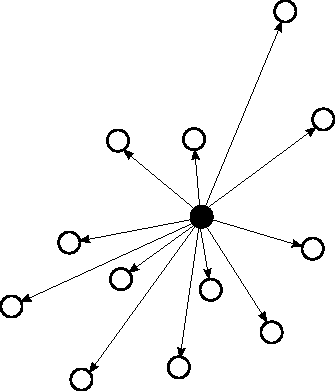
\includegraphics{figures/nbodies.pdf} \ecen
\caption{The na\"{\i}ve approach to the n body problem - calculate each interaction for each particle}
\end{figure}

The simplest solution to the N body problem is the basic $O(n^2)$ approach of calculating each interaction directly. Pseudocode for the algorithm is given below.\\

%%%%%PSEUDOCODE%%%%%%%%%
\begin{algorithm}[H]
 \SetLine
 \KwData{$r_i$: particle positions, $q_i$: particle charges, N: number of particles, Q: output array of charges}
 \For{i=0 to N}{
  \For{j=i to N}{
      \If{$i \not= j$}{
        $d := |r_i - r_j|$\;
        $Q[i] := q_i * q_j / d$\;
       }
  }
 }
 \caption{The basic approach to the N body problem}
\end{algorithm}

The advantages to the $O(n^2)$ approach are it's simplicity, ease of implementation, and it's low overhead. However, it's primary disadvantage is that it is limited to small numbers of particles by it's $O(n^2)$ complexity. These advantages and disadvantages are further discussed in Chapter \ref{chap:compare}

\subsection{Implementation analysis}
The $O(n^2)$ algorithm was run on increasing system sizes for one time step, and the time taken to calculate the potential at each atom's position was calculated. It is easy to turn this process into a dynamic simulation, using the relationship between potential energy, a particle's charge, and force.
%%%%%%%%FIGURE%%%%%%%%%%%%%
\begin{figure}[H]
\bcen 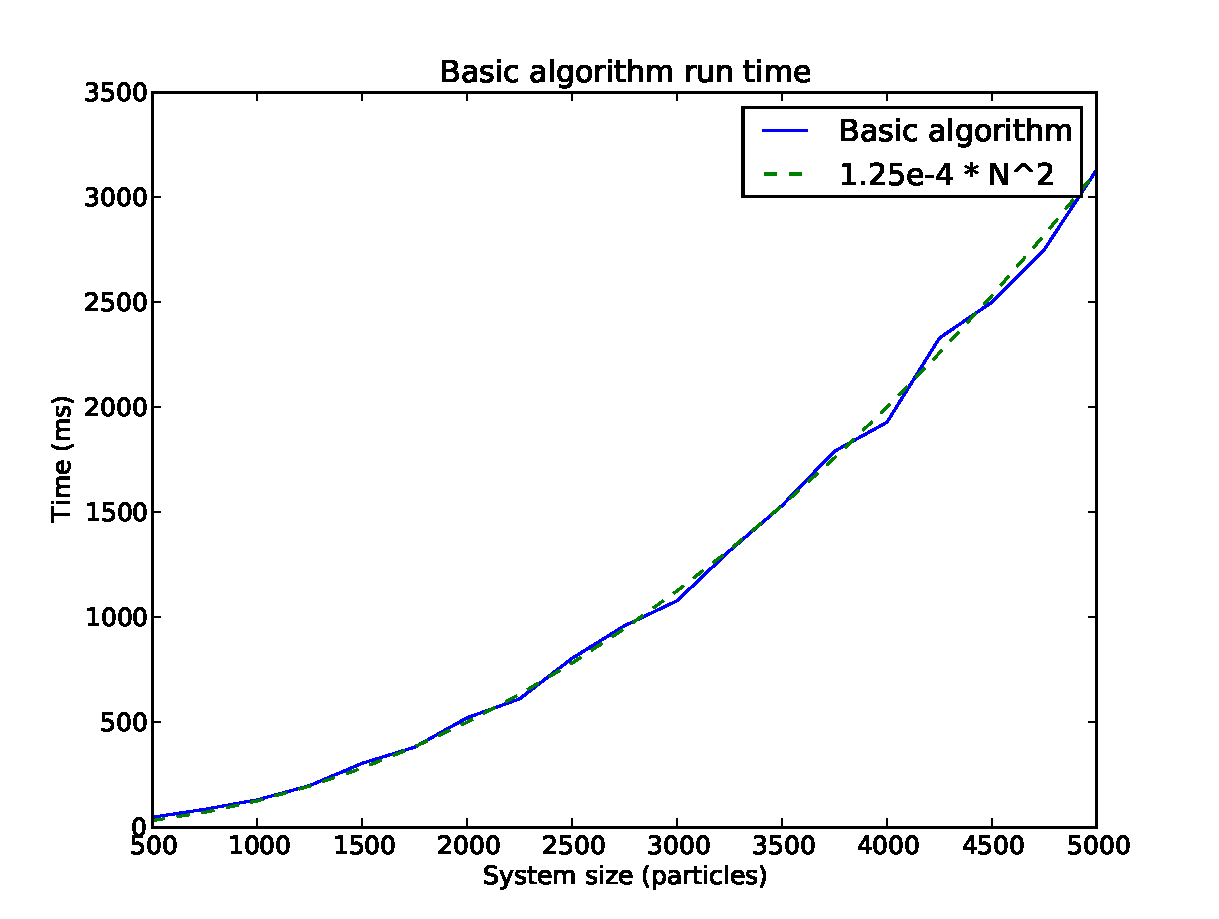
\includegraphics[width=0.75\textwidth]{figures/graphs/basic_algo_complex.pdf} \ecen
\caption{The basic algorithm's run time compared to a function of $N^2$. It is easy to see that the basic algorithms run time grows proportionally to $N^2$, as we would expect from it's complexity class $O(n^2)$}
\label{fig:basic_algo_complex}
\end{figure}

%_____________PME Section________________
\section{The particle mesh ewald method}
\subsection{Background}
\subsubsection{Potential vs. Energy}
Energy and potential are related but different concepts. They both describe effects charged particles have on their surrounding environment, however, \emph{Energy} is a property of a particle, and \emph{Potential} is a property of a field. \emph{Energy} is defined in terms of a particle-particle interaction, while \emph{Potential} describes a field from one charged particle.\\
Coulomb's law describes the potential from at $r_2$ from a charge $q_1$ at $r_1$ as 
\[V=\frac{1}{4\pi \epsilon_0} \frac{q_1}{|r_2 - r_1|}\]
And energy from a particle with charge $q_2$ at $r_2$ as $E = q_2 V$.\\
For our purposes, the constant term $\frac{1}{4\pi \epsilon_0}$ is material dependent, and is discarded.
\subsubsection{Ewald summation}
The key concept behind the \pmem{} is that of \emph{Ewald Summation}. Ewald Summation splits the energy between two particles into two components, the long range force and the short range force. \cite{petersen:3668}
\[
\phi(r) = \phi_{\text{sr}}(r) + \phi_{\text{lr}}(r)
\]
The advantage of doing this is that $\phi_{\text{sr}}$, the short range term, can be converges quickly in real space, while $\phi_{\text{lr}}$ converges quickly in reciprocal space. The \pmem{} takes advantage of this by calculating the $\phi_{\text{sr}}$ term by calculating potential directly for nearby particles, and uses a grid based direct fourier transformation to calculate the long range component.
\subsubsection{Real space computation}
The short range potential at a point can be computed by considering only particles within a small radius of the point. We can keep the radius small as $\phi_{\text{sr}}$ converges quickly in real space. This is also important, as we need to keep the number of particles considered less than $N$, in order to reduce the algorithm from $O(n^2)$ complexity. This is the case though, as the radius we consider is constant and less than the size of the simulation cell width, and we assume the particles are distributed randomly within the simulation cell.
%%%%%%%%FIGURE%%%%%%%%%%%%%
\begin{figure}[H]
\bcen 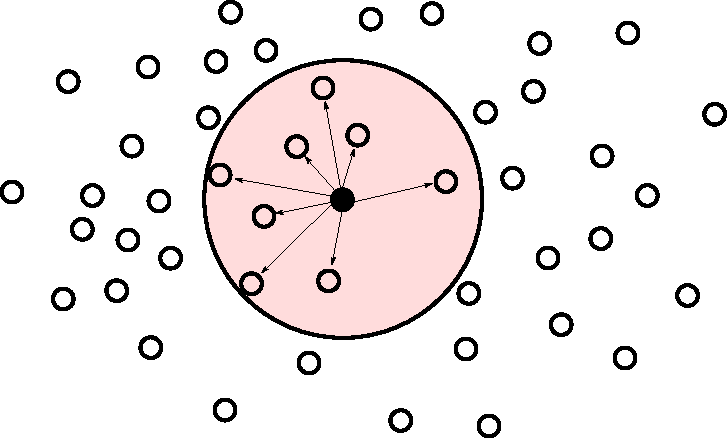
\includegraphics{figures/cutoff.pdf} \ecen
\caption{A particle and the particles that we consider it's interactions with, based on the cutoff distance}
\end{figure}

\subsubsection{Reciprocal space computation}
The reciprocal space is the long range part of the potential computation, and which converges slowly in real space. However, in reciprocal space, it converges quickly, so we use discrete fourier transformations to calculate this part of the sum.\\

Discrete fourier transformations require a discrete space to transform, however, our real space is continuous. So for this, we need to discretise the charges onto a grid. The approach taken in the original paper was to use Lagrangian interpolation to achieve this. Close mesh cells receive most of the charge from each particle, and this amount decreases to zero at some point, depending on the interpolation order. This is described in detail in Section \ref{sec:math_desc_lagrange}.\\
%%%%%%%%FIGURE%%%%%%%%%%%%%
\begin{figure}[H]
\bcen 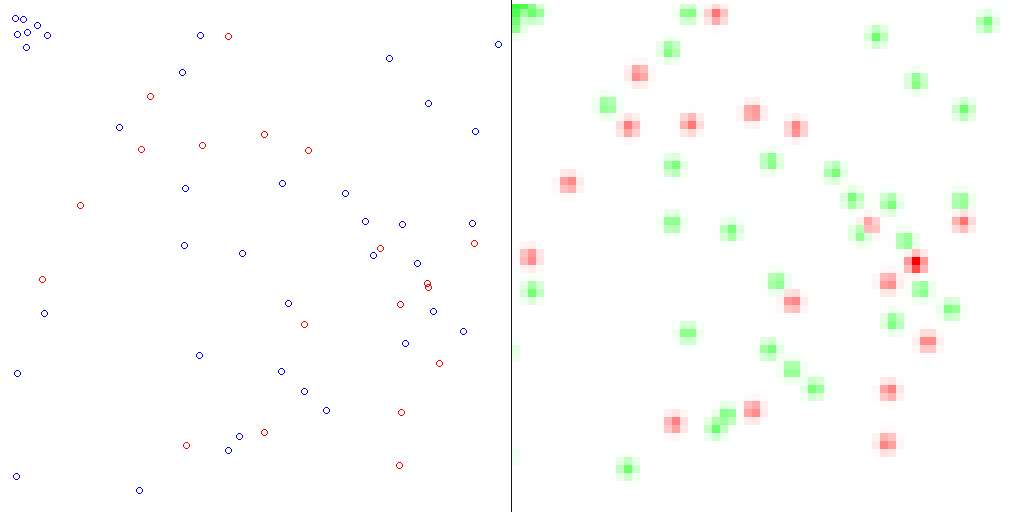
\includegraphics[width=\textwidth]{figures/Qarray.jpg} \ecen
\caption{A distribution of continuous charges, and an interpretation of them as discrete charges}
\end{figure}

An alternative to using lagrange interpolation is to use cardinal B splines. This modification is known as the \emph{Smooth Particle Mesh Ewald} method, and is advantageous in terms of accuracy, and is also easily differentiable, which is important if the forces are required as well as the potentials.  \cite{essmann:8577} This is the method that was implemented in this paper.


\subsubsection{Periodic boundary conditions}
One advantage that the Particle Mesh Ewald method has is the ability to simulate \emph{Periodic Boundary Conditions} \cite{essmann:8577}. Periodic Boundary Conditions have a wrap around behaviour - that is, instead of treating the walls of the simulation unit as empty space, we can allow them to loop around to the other side of the box again, effectively allowing infinite replication of the simulation unit. This is helpful practically, as many applications are interested in the effects on a small portion of a large system \cite{toukmaji:73} (For example, simulation of water at a molecular scale). Simulating the entire system would be time consuming if not impossible, and simulating only a small portion without Periodic Boundary Conditions would produce unrealistic results (Molecules may disperse into empty space over time). While useful practically, Periodic Boundary Conditions do not change the complexity or performance, and as our interest is in a comparison with the \fma{}, we do not implement Periodic Boundary Conditions in this paper.
%%%%%%%%FIGURE%%%%%%%%%%%%%
\begin{figure}[H]
\bcen 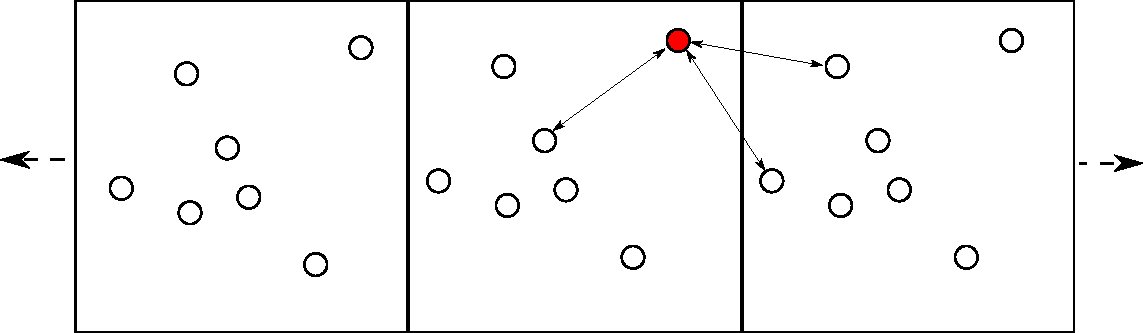
\includegraphics[width=0.75\textwidth]{figures/pbc.pdf} \ecen
\caption{A particle (in red) interacting with it's nearest neighbours, with periodic boundary conditions in one dimension (x axis)}
\end{figure}

\subsection{Mathematical description}
\subsubsection{Interpolating the charges to the Q array}
\label{sec:math_desc_lagrange}
We first present the formulation of the Q array based on lagrangian interpolation. 
\begin{equation} \label{eq:q_array}
Q(k_x,k_y) = \sum_{i=1} ^N q_i W_{2p}(u_{xi} - k_x) * W_{2p}(u_{yi} - k_y)
\end{equation}
Where $N$ is the number of particles,\\
$n_1,n_2$ are integers $< N$,\\
$W_{2p}$ is a Lagrangian polynomial of order $p$ with a value in the range $[0,1]$,\\
$K$ is the number of cells we split the grid into,\\
$u_{xi}, u_{yi}$ are scaled fractional coordinates of particle $i$ (Scaled fractional coordinate coordinates meaning $u_{xi} = K * (r_{xi} / (\text{simulation width}))$, $r_{xi}$ is the particle i's $x$ coordiante, so $0 \leq u_{xi} \leq K$).\\
More information can be found in \cite{essmann:8577}\\

We can replace $W_{2p}$ in the above with $M_n$, a cardinal B spline of order $n$, and the formulation of the Q array is the same. This modification is known as the Smooth \pmem{}. From this point forward, we will use cardinal B spline interpolation.


\subsubsection{Calculating electrostatic potential from the Q array}
With this Q array we can calculate the long range contribution to the electrostatic potential in reciprocal space.\\
The reciprocal space contribution to the electrostatic energy can be written as,\\
\begin{equation}
E_{\text{rec}} = \frac{1}{2*\pi*V} \sum_{m \not= 0} \frac{\text{exp}(- \pi^2 m^2 / \beta^2)}{m^2} B(m_1,m_2) S(m) S(-m)
  \label{eq:primitive_rec_energy} \end{equation}
Where $V$ is the volume (or in the two dimensional case, area) of the simulation cell,\\
$\beta$ is the ewald coefficient,\\
$S$ is the structure factor.\\
$B$ is the matrix of B spline inverse fourier transform moduli, $B(m_1,m_2) = |b_1(m_1)|^2 * |b_2(m_2)|^2$. More detail on this can be found in \cite{essmann:8577}.\\
It is shown in \cite{essmann:8577} that $S(m) \approx F(Q(m))$, so we can rewrite this as a convolution\\
\begin{equation}
E_{\text{rec}} = \frac{1}{2} \sum_{m_1 = 0}^K \sum_{m_2 = 0}^K Q(m_1,m_2) * (\theta_{\text{rec}} \star Q)(m_1,m_2)
\label{eq:energy_rec}
\end{equation}
With $\theta_{\text{rec}} = F(B * C)$, and so $(\theta_{\text{rec}} \star Q)(m_1,m_2) = F(B * C * F^{-1}(Q))$ \cite{essmann:8577} \cite{lee05}\\
Where $C$ is the matrix for the original exponential term from Equation \ref{eq:primitive_rec_energy}, that is,
 \bcen$\displaystyle
C(m_1,m_2) = \frac{1}{\pi V} \frac{\text{exp}(- \pi^2 m^2 / \beta^2)}{m^2} $ for $ m \not= 0, C(0,0) = 0
$\ecen 

\subsubsection{Interpolating energies back from the grid in real space}
\label{sec:interpolate_from_grid}
If we have a point $r$ in real space that we wish to calculate the potential for, we can interpolate back from a mesh in the same way we did while creating the discrete mesh.
That is, with $r = (r_x,r_y)$, which has scaled fractional coordinates $(u_x,u_y)$ (see Section \ref{sec:math_desc_lagrange}), at point $r$ we have\\
\begin{equation}
\label{eq:interpoalte_from_grid}
E(r_x,r_y) = \sum _{i,j = -n} ^{n} Q(\lfloor u_{x+i} \rfloor,\lfloor u_{y+j} \rfloor) * M_n(u_x - \lfloor u_{x+i} \rfloor) * M_n(u_y - \lfloor u_{y+j} \rfloor)
\end{equation}
This equation iterates over cells within our interpolation order $n$, and calculates the weighting we ascribe to the cell ($ M_n(u_x - \lfloor u_{x+i} \rfloor) * M_n(u_y - \lfloor u_{y+j} \rfloor$, a real number in the range $[0,1]$). Summing the proportion of the grid charge assignments, we produce B Spline interpolated values from the grid.
\subsubsection{The ewald coefficient}
The ewald coefficient, $\beta$, is a number describing the ratio between the real space and the reciprocal space contributions to the calculation of the total energy. In practice, it depends on the tolerance $\epsilon_\text{tol}$, and our desired cutoff distance $r_{\text{cut}}$ in the following way, \cite{darden:10089} \cite{essmann:8577}\\
\begin{equation}
\frac{\text{erfc}(\beta r_{\text{cut}})}{r_\text{cut}} \leq \epsilon_\text{tol}
\label{eq:ewald_coeff}
\end{equation}
Where erfc is the complimentary error function, a function that tends quickly to zero, depending on it's argument. The relation means that for $r > r_{cut}$, we have $\frac{\text{erfc}(\beta r_{\text{cut}})}{r_\text{cut}} \leq \epsilon_\text{tol}$, and for all $r > r_\text{cut}$ we can ignore the direct energy contribution, given by equation \ref{eq:energy_dir} \cite{essmann:8577}\\
\begin{equation}
E_\text{dir} = \frac{1}{2} \sum_{n} \sum_{i,j = 1} ^N \frac{q_i q_j \text{erfc}{\beta |r_j - r_i|}}{|r_j - r_i|}
\label{eq:energy_dir}
\end{equation}
Which becomes approximately
\begin{equation}
E_\text{dir} \approx \frac{1}{2} \sum_{n} \sum_{i,j = 1} ^{\overset{*}{N}} \frac{q_i q_j}{|r_j - r_i|}
\label{eq:energy_dir_noerfc}
\end{equation}
Where the $*$ indicates terms with $|r_j - r_i| > r_{\text{cut}}$ are left out of the sum





\subsection{The algorithm}
\subsubsection{Main particle mesh ewald flow}
The basic flow of the algorithm is given below\\ \newline
%%%%%PSEUDOCODE%%%%%%%%%
\begin{algorithm}[H]
\SetLine
\KwData{$Q$: Charge assignment matrix, $r_{\text{cut}}$: Cutoff distance, $r$: position at which we calculate the potential}
Initialise the ewald coefficient (Equation \ref{eq:ewald_coeff})\\
Calculate the B spline coefficients (Details in \cite{essmann:8577} \cite{lee05})\\
Allocate particles to their cells (Section \ref{sec:verlet})\\
Initialise the Q matrix (Equation \ref{eq:q_array})\\
Calculate reciprocal energy (Equation \ref{eq:energy_rec})\\
Calculate direct energy (Equation \ref{eq:energy_dir})\\
Interpolate reciprocal energies back to desired coordinates (Section \ref{sec:interpolate_from_grid})\\
\For{Every particle $p$ within $r_{\text{cut}}$ of $r$ (Calculate using Verlet list, (Section \ref{sec:verlet})}{
Caclulate and sum the direct potential from $p$ at $r$.
}
Combine the interpolated energy and directly computed energy
\end{algorithm}

\subsubsection{Verlet list algorithm}
\label{sec:verlet}
The following algorithm utilises a list known as a \emph{Verlet list} to keep track of which particles are within a cutoff distance of each other, with only $O(n)$ complexity. It is used in the direct energy calculation of the \pmem{}\\
%%%%%PSEUDOCODE%%%%%%%%%
\begin{algorithm}[H]
\SetLine
\For{i=0 to N}{
    $\text{cell}_x := \lceil u_{xi} \rceil$; (With $u_{xi}$ the scaled fractional x coordinate, as defined in Equation \ref{eq:q_array}))\\
    $\text{cell}_y := \lceil u_{yi} \rceil$; (With $u_{yi}$ the scaled fractional y coordinate))\\
    $\text{direct range} := \lceil r_{cut} / \text{mesh cell width} \rceil$\\
    \For{$\delta_x = -\text{direct range}$ to $+\text{direct range}$}{
        \For{$\delta_y = -\text{direct range}$ to $+\text{direct range}$}{
            \If{$\text{cell}_x + \delta_x$ and $\text{cell}_y + \delta_y$ are in the mesh}{
                Add i to the array closeParticles[$\text{cell}_x + \delta_x$][$\text{cell}_y + \delta_y$]
            }
        }
    }
}
\end{algorithm}
After this, the array closeParticles[x][y] contains all particles within $r_cut$ distance from a particle contained in mesh cell $x,y$.

\subsection{The implementation}
The \pmem{} method was implemented in Java, with a GUI front end. In this section, we break down the \pmem{}, and look at the interesting data structures and methods used in initialisation and potential calculations.

\subsubsection{The Cardinal B Spline}
The Cardinal B Spline was implemented by means of recursion. The class \texttt{BSpline.java} contains the methods required for evaluating the B Spline and it's derivative, as well as the Euler Exponential splines (the B matrix in Eq. \ref{eq:primitive_rec_energy}). This recursion is performed many times, and is costly at high accuracies (high B Spline orders). This makes it a target for optimisation (See section \ref{sec:optimisations})
\subsubsection{Calculating the ewald coefficient}
The ewald coefficient is calculated by means of a binary search for a coefficient that satisfies the inequality in Eq. \ref{eq:ewald_coeff} as closely as it can according to $\epsilon_{\text{tol}}$. So we look for the $\beta$ that minimizes
\[
\left| \frac{\text{erfc}(\beta * r_{\text{cut}})}{r_\text{cut}} - \epsilon_\text{tol} \right| 
\]
In a binary search
\subsubsection{Fast Fourier Transformations}
The chosen library for Fast Fourier Transformations (Required for calculation of the reciprocal space potential) was the JTransforms library. \cite{JTransform}. This library has the advantage of being implemented in pure Java code, allowing simpler integration and debugging. The Fourier Transformation operation is the core of the run time for the \pmem{}, and so and optimised library is essential for performance reasons.
\subsection{Running time analysis}
\subsection{Accuracy analysis}
\label{sec:optimisations}
%_________________ FMA SECTION __________________
\section{The Fast multipole algorithm}
\subsection{Background}
The \fma{} is similar to the \pmem{} in that both use a grid structure, and bounded approximations, to speed up computation. However, they are different in the ways they use the mesh, and the approximations that are made.
\subsubsection{Complex plane}
It should be noted that for this algorithm, it is simplest to implement in two dimensions. It is possible to to implement in three dimensions, with Spherical Harmonics \cite{Ihler04}, however this is not discussed in this paper. Instead, we work in two dimensions, on the complex plane. We give a point $(x,y)$ on the Real plane the value $z = x + yi$ on the Complex plane. This way, we can represent each point as a single number, and use complex versions of functions while calculating the multipole expansions.

\subsubsection{Multipole expansions}
A multipole expansion is a function which is a sum of a series of terms, which converges to some other function (in this case, the potential energy function). This convergence is fast, which makes it a good approximation to use in the \fma{}. These multipole expansions are centered on one point, and are valid for points within a certain distance of this center, but may be shifted and combined to gain more general multipole expansions. \cite{greengard:315}

\subsubsection{The mesh}
The mesh is similar to the one used in the \pmem{}. We say that the mesh has $n$ levels, and at each level we split each cell into quarters, starting with level $0$, which is the simulation cell. Each cell is split in four when moving down a level. We call the four sub cells of a cell $c$ the \emph{children} of $c$. Conversely, we call the cell that $c$ is a sub cell of the \emph{parent} of $c$.
%%%%%%%%FIGURE%%%%%%%%%%%%%
\begin{figure}[H]
\bcen 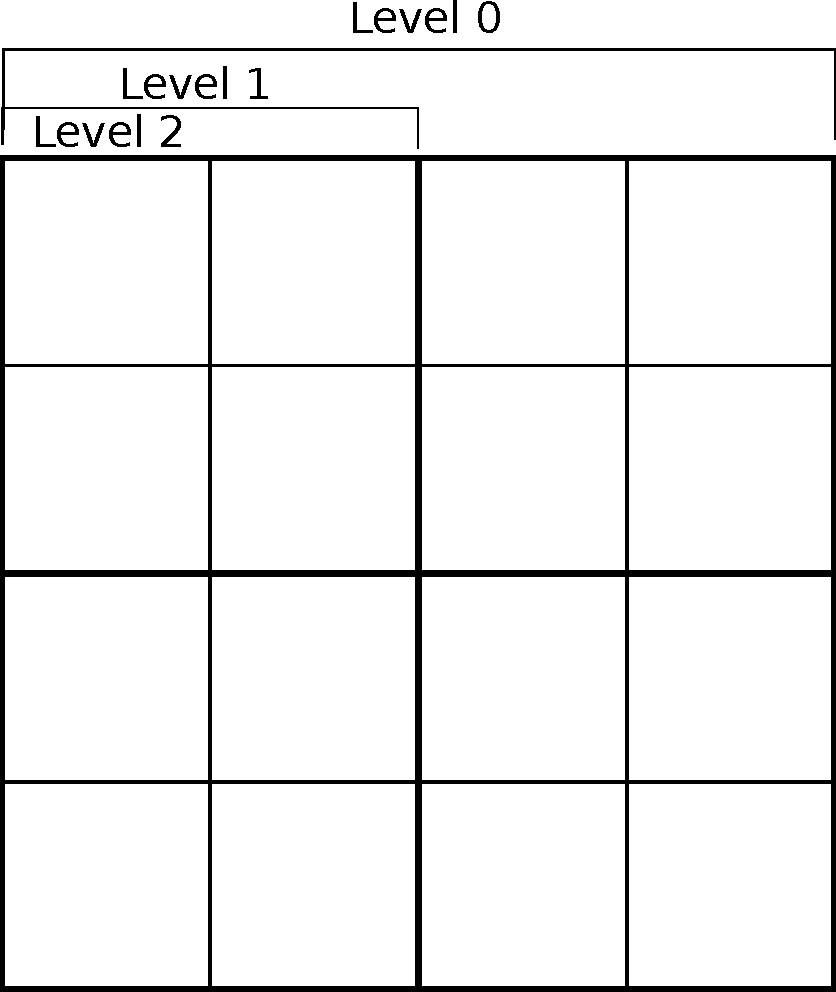
\includegraphics[width=0.35\textwidth]{figures/fma_mesh.pdf} \ecen
\caption{A simulation cell, with meshes up to level 2 displayed, giving $2^n = 2^2 = 4$ boxes per side}
\end{figure}

\subsubsection{Well separated cells}
\label{sec:well_sep}
For a cell $c$, we call a cell $d$ \emph{Well separated} from $c$ if\\
1) $\text{Parent}(d)$ is adjacent to $\text{Parent}(c)$ (adjacent horizontally, vertically or diagonally)\\
2) $d$ is not adjacet to $c$\\
\newline
These \emph{well separated} cells are the ones which we will use the expansions to calculate potential for. For cells that are not well separated, we will calculate interactions directly.
%%%%%%%%FIGURE%%%%%%%%%%%%%
\begin{figure}[H]
\bcen 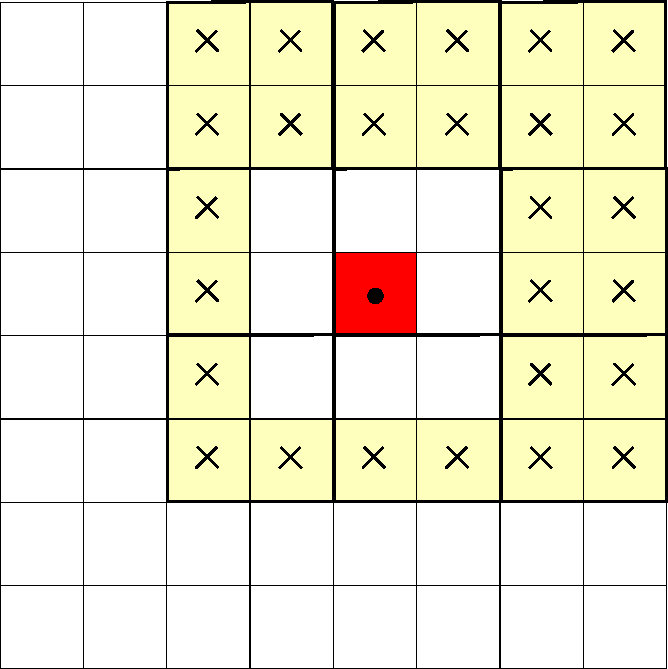
\includegraphics[width=0.35\textwidth]{figures/wellsep.pdf} \ecen
\caption{A cell, marked with a circle, and the squares that are well separated from it, marked with crosses.}
\end{figure}

\subsection{Mathematical description}
\label{sec:fma_math}
\subsubsection{Potential and the multipole expansion approximation}
We describe the potential at a point $x_0 \in \mathbb{C}$ from the charge $q$ at $x \in \mathbb{C}$ by
\begin{equation}
\phi_{x_0} = -q\text{log}{|x - x_0|}
\label{eq:potential}
\end{equation}
A multipole expansion for this function is derived in \cite{greengard:315}. Suppose that $m$ charges of strength $\{q_i,i=1,...,m\}$ are located at points $\{z_i, i=1,...,m\}$, with $|z_i| < r$. Then for any $z \in \mathbb{C}$ with $|z| > r$, the potential $\phi(z)$ is given by
\begin{equation}
\phi(z) = Q \text{log}(z) + \sum_{k=1} ^{\infty} \frac{a_k}{z^k}
\label{eq:multipole_expansion}
\end{equation}
Where
\begin{equation}
Q = \sum_{i=1} ^m q_i 
\hspace{0.5cm} \text{and} \hspace{0.5cm}
a_k = \sum_{i=1} ^m \frac{-q_i z^k _i}{k}
\end{equation}
While this is exact for an infinite sum of terms, we can truncate the series at term $p$, and if $p$ is large enough, this approximation is close to the actual potential $\phi(z)$. A description of how close can be found in \cite{greengard:315}
\subsubsection{Shifting multipole expansions}
A multipole expansion's center may be shifted, which is necessary for the \fma{}. Suppose that
\begin{equation}
\phi(z) = a_0 \text{log}(z-z_0) + \sum_{k=1} ^{\infty} \frac{a_k}{(z-z_0)^k}
\label{eq:pre_shift_multipole}
\end{equation}
Describes a multipole expansion which is centered on $z_0$. We can then shift this multipole expansion to be centered at the origin,
\begin{equation}
\phi(z) = a_0 \text{log}(z) + \sum_{l=1} ^{\infty} \frac{b_l}{z^l}
\label{eq:shifted_multipole}
\end{equation}
Where
\begin{equation}
b_l = \left(\sum_{k=1} ^l a_k z_0^{l-k} \binom{l-1}{k-1} - \frac{a_0 z_0^l}{l} \right)
\label{eq:b_descr}
\end{equation}
Note that this procedure of shifting to the origin is equivalent to shifting from any point $a$ to point $b$, if we treat point $b$ as the origin, and $a-b$ as our previous multipole expansion center.
\subsubsection{Local expansions}
We can find a local expansion about the origin due to a set of charges within radius $R$ of $z_0$, with $|z_0| > (c+1)R, \hs c > 1$. This local expansion is based on the multipole expansion at the same point.
\begin{equation}
\phi(z) = \sum _{l=0} ^{\infty} b_l * z^l
\label{local_expansion}
\end{equation}
Where
\begin{equation}
b_0 = \sum_{k=1} ^{\infty} \frac{a^k}{z^k_0} (-1)^k + a_0 \log(-z_0)
\label{where_local_expansion}
\end{equation}


\subsection{The algorithm}
\label{sec:fma_alg}
The basic flow of the algorithm is given below\\
%%%%%PSEUDOCODE%%%%%%%%%
\begin{algorithm}[H]
\SetLine
\KwData{level-count: the number of mesh levels we create, $P$: the set of particles, $r$: a point at which we wish to calculate the potential}
\For{i=0 to level-count}{Initialise mesh[i] by adding all particles $p \in P$ to the appropriate cells}
\For{Each cell $c$ in mesh[level-count]}{Form a multipole expansion at at $c$, using Equation \ref{eq:multipole_expansion}}
\For{i=(levelcount-1) down to 0}{
    \For{Each cell $c$ in mesh[i]}{
        Shift each multipole expansion for the child cells of $c$ (in mesh[i+1]) to $c$ (Eq. \ref{eq:shifted_multipole})\;
        Combine and save these multipole expansions by addition\;
     }
}
\For{Each cell $c$ in mesh[0]}{
        Form a local expansion at $c$ based on $c$'s multipole expansion\;
        Shift $c$'s local expansion to the children of $c$\;
 }
\For{i=1 to level-count}{
    \For{Each cell $c$ in mesh[i]}{
        Shift $c$'s local expansion to the children of $c$\;
    }
}
Set the cumulative potential to 0\;
\For{Each cell $c$ in mesh[level-count]}{
    \eIf{$c$ is Well Separated from $d$'s cell}{
        Calculate the potential at $r$ from $c$'s local expansion\;
        Add this potential to the cumulative potential\;
    }{
        Calculate the potential at $r$ from $c$'s particles directly\;
        Add this potential to the cumulative potential\;
    }
}
Return the cumulative potential\;
\end{algorithm}

\subsection{The implementation}
A more object oriented approach was taken in the implementation of the \fma{} than in the \pmem{}. The primary classes the mathematics are \texttt{LocalExpansion.java} and \texttt{MultipoleExpansion.java}, which contain methods for creating, shifting, evaluating and storing the expansions described in Section \ref{sec:fma_math}.\\

An object for a mesh is implemented in \texttt{Mesh.java}, which contains a 2D array of cells, defined in \texttt{Cell.java}. The \texttt{Mesh} class contains a function called \texttt{makeCoarserMesh()} which creates a coarser mesh, shifting and merging multipole expansion in the process. This coarser mesh is saved into an array of each mesh level, from the maximum depth, to zero.

\subsection{Running time analysis}
The \fma{} was run over the class of problems with sizes in the range [0,5000] with an increment of 250, and [0, 20000] with an increment of 1000. The results are shown in Figure \ref{fig:fma_complex}.
%%%%%%%%FIGURE%%%%%%%%%%%%%
\begin{figure}[H]
\subfigure[Range 0 - 2000]{ \label{fig:fma_complex_a} 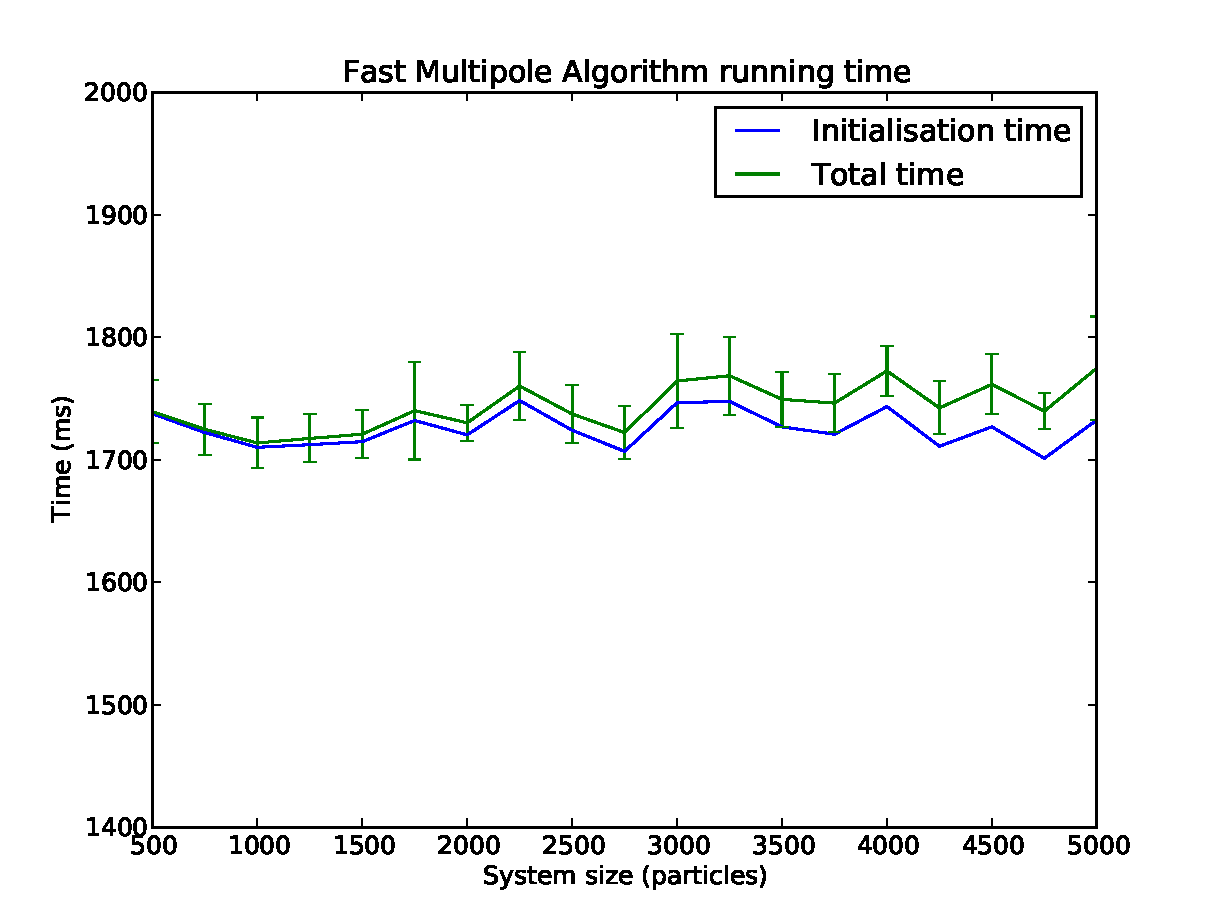
\includegraphics[width=0.49\textwidth]{figures/graphs/fma_0_5000.pdf}}
\subfigure[Range 0 - 20,000]{\label{fig:fma_complex_b} 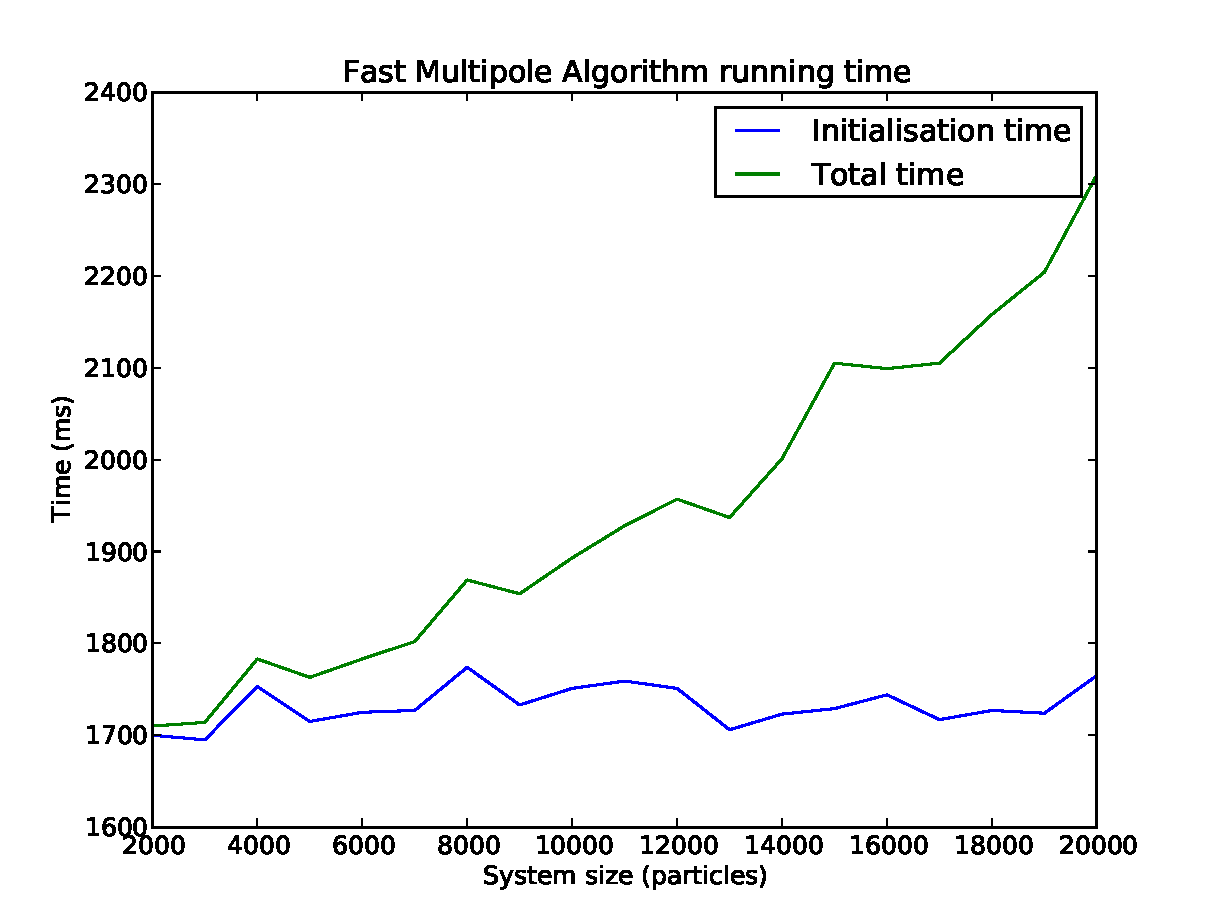
\includegraphics[width=0.49\textwidth]{figures/graphs/fma_2k_20k.pdf}}
\caption{The \fma's performance over the group of systems in the range 0 to 5,000 particles, and 0 to 20,000.}
\label{fig:fma_complex}
\end{figure}

The graphs here show the initialisation time and total time for the \fma{} on a set of problems. The initialisation time is the time required to compute the multipole and local expansions, and the total time is the initialisation time, with the time taken to evaluate these expansions included.

Figure \ref{fig:fma_complex_a} shows the same range as Figure \ref{fig:basic_algo_complex}, the basic algorithm's complexity. In it, we see that the initialisation time is taking most of the computation time. Each data point is an average of 20 trials, with the error bar indicating the standard deviation.

Figure \ref{fig:fma_complex_b} shows the \fma's run time for much larger problems, with up to 20,000 particles. We can see the initialisation time stay constant, while the total time grows linearly. So, we confirm that our implementation of the \fma is in the complexity class $O(n)$ \newline

Using \texttt{VisualVM} \cite{VisualVM}, the table below of running times spent in each method was produced.

\begin{table}[H]
    \begin{tabular}{|l|l|l|}
        Method                       & Proportion of running time & Method description \\ \hline
        \texttt{fma.LocalExpansion()}         & 31.6\%                      & Local expansion initialisation        \\ 
        \texttt{math.Complex.power()}         & 27.8\%                      & Calculates $c^x$             \\ 
        \texttt{math.Complex.ln()}            & 24.9\%                      & Calculates $\text{log}(c)$ \\
        \texttt{math.Binomial.binomial()}     & 9.6\%                       & Calculates binomial function \\ 
        \texttt{fma.MultipoleExpansion.add()} & 1\%                         & Adds multipole expansions
    \end{tabular}
    \label{tab:time_breakdown}
    \caption{The proportion of the running time spent in each method for the \fma while benchmarking.}
\end{table}

We can see that most of the running time is spent forming local expansions, and doing complex arithmetic. The run time is split over several different methods, which indicates there are no severe efficiency concerns. Most of the run time is spent performing complex arithmetic, which is what should be expected.

\subsection{Accuracy analysis}
The \fma has two main parameters that control accuracy - the number of mesh levels, and the number of terms in the multipole expansion. We call the number of mesh levels $N$ and the number of terms in the multipole expansion $p$. For reasonable accuracy, we should expect $N \approx \text{log}_4(N)$ and $p \approx \text{log}_2(\epsilon)$, where $\epsilon$ is the desired precision. \cite{greengard:315}
\subsubsection{Maximum mesh level}
We plot the accuracy of the method as a function of these two parameters. In figures \ref{fig:fma_mesh_acc} and \ref{fig:fma_fixed_mesh_acc}, we demonstrate the effect the mesh level has on the error. 

%%%%%%%%FIGURE%%%%%%%%%%%%%
\begin{figure}[H]
\bcen 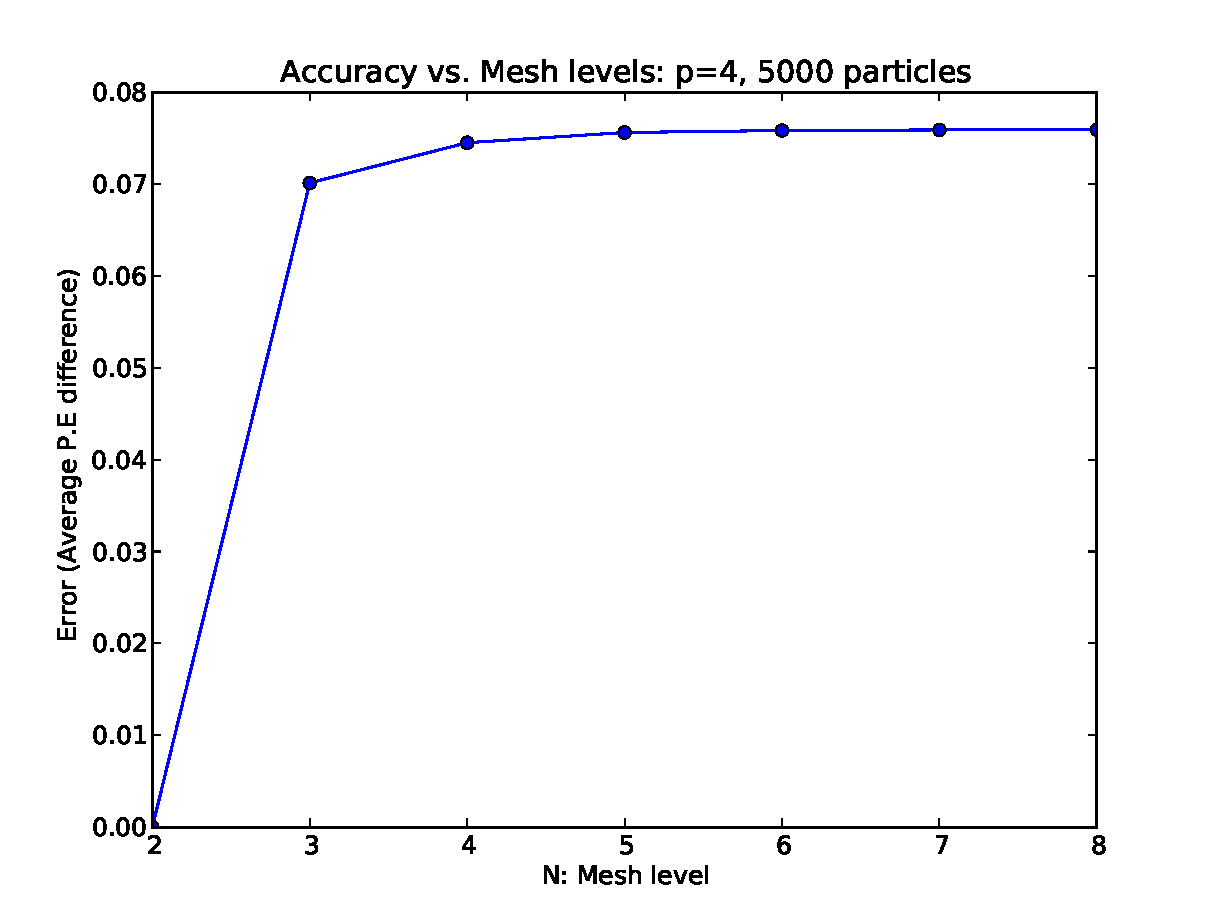
\includegraphics[width=0.75\textwidth]{figures/graphs/fma_mesh_acc.pdf} \ecen
\caption{The relationship between $N$, mesh levels, and the error, when comparied with the basic algorithm.}
\label{fig:fma_mesh_acc}
\end{figure}

Figure \ref{fig:fma_mesh_acc} shows the error \emph{increasing} with mesh level. This seems counter intuitive, however, according to The \fma algorithm from Section \ref{sec:fma_alg}, we calculate interactions directly for cells that are not Well separated (See Section \ref{sec:well_sep}). With low mesh levels, such as $N=2$, this would include the entire simulation unit, which leads to the error of 0 we see at $N=2$. Increasing from here, we see the error level out to approximately 0.075. This graph shows that increasing Mesh level does not necessarily lead to improved accuracy.

%%%%%%%%FIGURE%%%%%%%%%%%%%
\begin{figure}[H]
\bcen 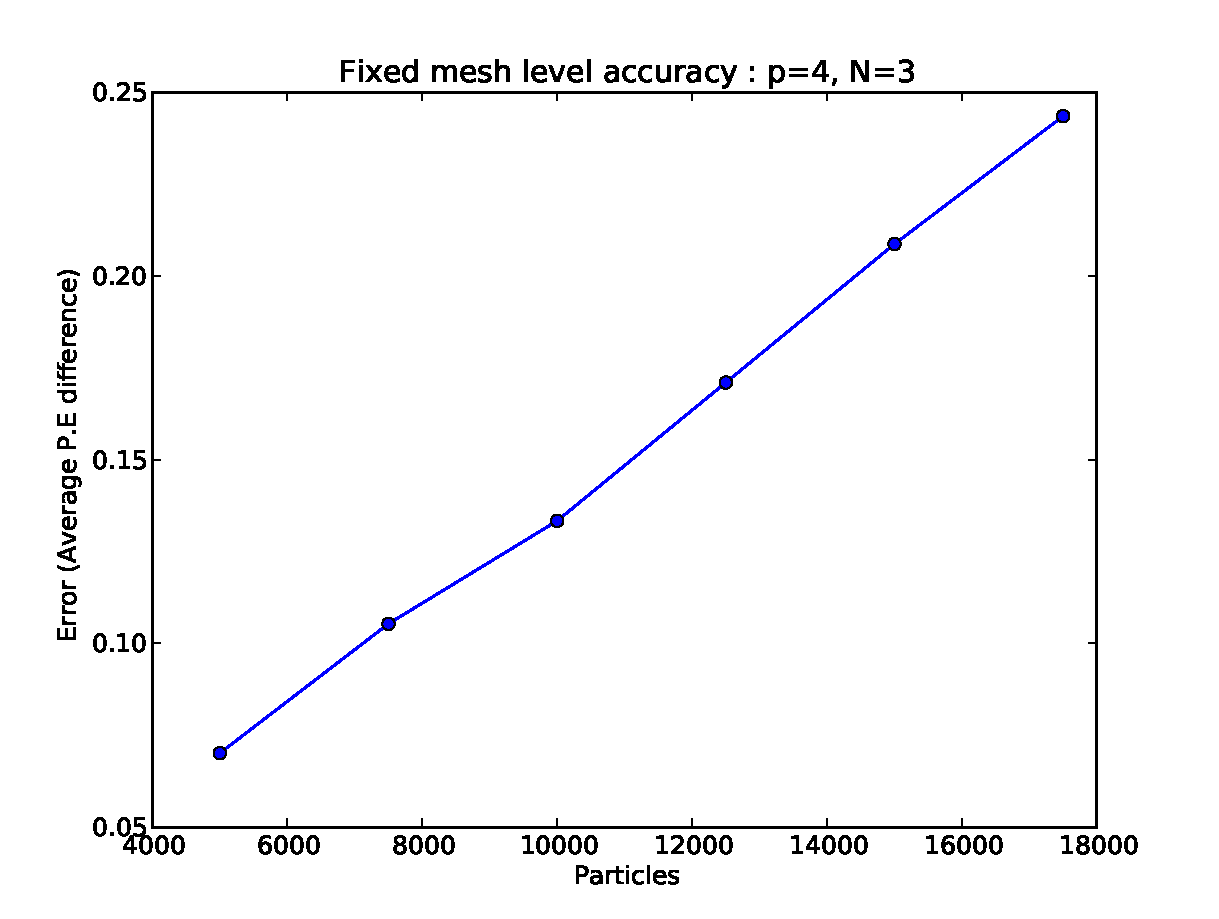
\includegraphics[width=0.75\textwidth]{figures/graphs/fma_fixed_mesh_acc.pdf} \ecen
\caption{The error for the \fma with a fixed mesh level $N=3$, with an increasing system size}
\label{fig:fma_fixed_mesh_acc}
\end{figure}

Figure \ref{fig:fma_fixed_mesh_acc} above, shows the effect of an increasing system size for a fixed $N$. We can see that the error grows linearly as we increase the number of particles if we keep $N$ and $p$ constant. From this we can confirm that a good rule is $N \approx \text{log}_4(n)$, with $n$ being the total number of particles in our system. This is recommended, as it keeps the number of particles per cell approximately constant. %TODO: a graph could show this.

\subsubsection{Number of terms}
Next we examine the effect the number of terms we truncate our multipole expansion at, $p$, has on the accuracy of our simulation.
%%%%%%%%FIGURE%%%%%%%%%%%%%
\begin{figure}[H]
\bcen 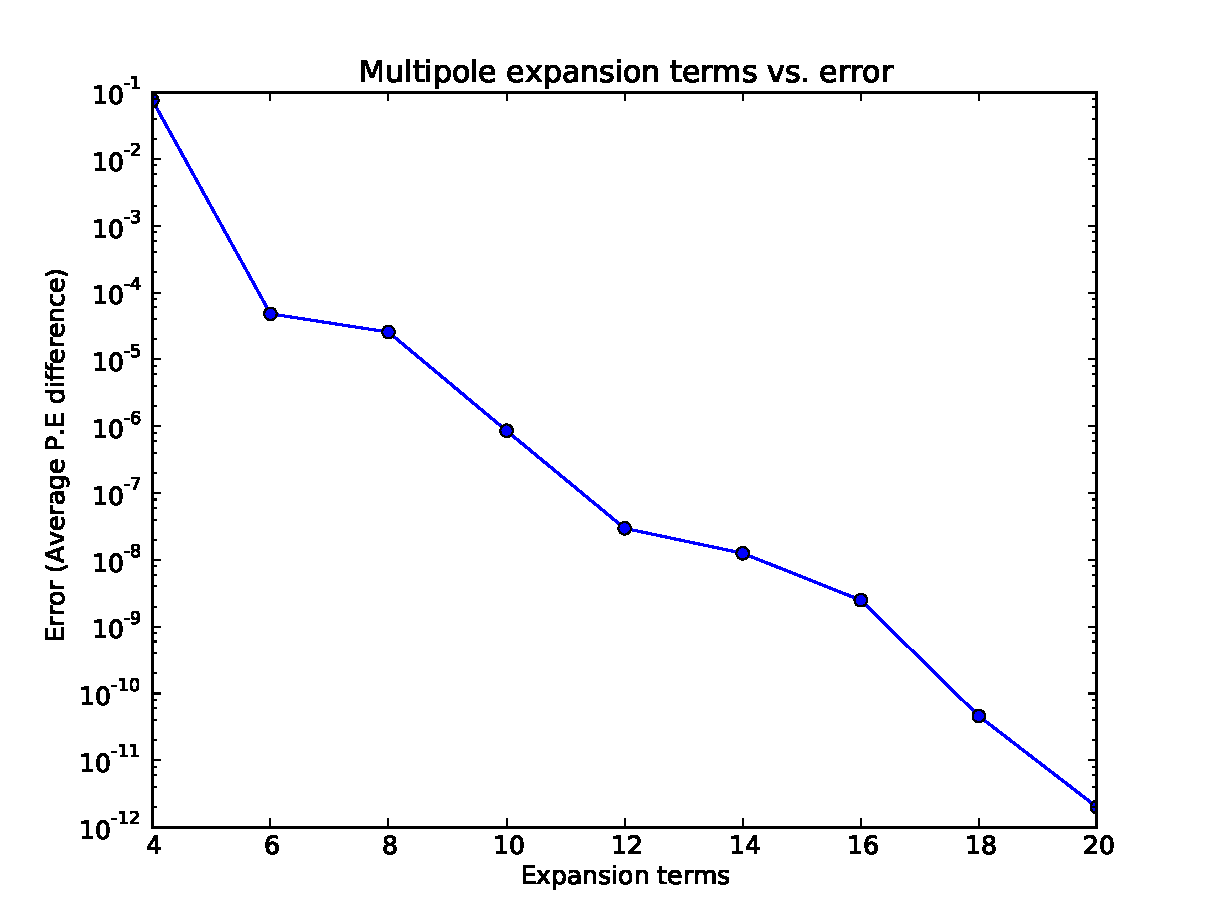
\includegraphics[width=0.65\textwidth]{figures/graphs/fma_terms_acc.pdf} \ecen
\caption{The error, on a logarithmic scale, vs. the number of terms in the multipole expansion, with a system size of is 5000 particles}
\label{fig:fma_terms_acc}
\end{figure}

From figure \ref{fig:fma_terms_acc} we see that the accuracy of the \fma increases exponentially as we increase the number of terms in our expansion. The improvement in accuracy as we increase the number of expansion terms decreases after $N \approx 20$, however, as we approach the machine precision.

%TODO: show the effect these parameters have on the running time?

\chapter{Comparison of the algorithms}
\label{chap:compare}
\chapter{Discussion}

\bibliographystyle{plain}	
\bibliography{references}	

\end{document}
